\section{Introduction}


\begin{frame}
 \slideheading{What is odeint?}

 ODE -- ordinary differential equation

 int -- Integration

 A C++ library for solving ordinary differential equations

 {\tt odeint.com}

\end{frame}

\begin{frame}
 
 \slideheading{What is an ODE?}

 Vielleicht Marios Folie(n) kopieren

\end{frame}


\begin{frame}[fragile]
 
 \slideheading{Who uses odeint}

netevo

ompl (Open Motion planning library)

\dots

\end{frame}





\frame{
  \frametitle{The interface problem in C/C++}
  
    \begin{itemize}
      \item Many frameworks exist to do numerical computations.
      \item Data has to be stored in containers or collections.
      \item GSL: {\tt gsl\_vector}, {\tt gsl\_matrix}
      \item NR: pointers with Fortran-style indexing
      \item Blitz++, MTL4, boost::ublas
      \item QT: {\tt QVector}, wxWidgets: {\tt wxArray}, MFC: {\tt CArray}
    \end{itemize}

  %\vspace{2ex}

    {\bf \color{red} But:} All books on C++ recommend the use of the STL containers {\tt std::vector},
    {\tt std::list}, \dots

 \pause

  %\vspace{2ex}

  \begin{block}{Theoretical solution of the interface mess}
  GoF Design Pattern: Adaptor, also known as Wrapper

  % {\tiny Gamma, Holm, Johnson, Vlissides: {\it Design Patterns, Elements of Reuseable Object-Oriented Software},  1998.}
  \end{block}

  \pause

  \begin{exampleblock}{Alternative}
   Generic, container independent algorithms
  \end{exampleblock}

}

\frame{
  \frametitle{Example}
  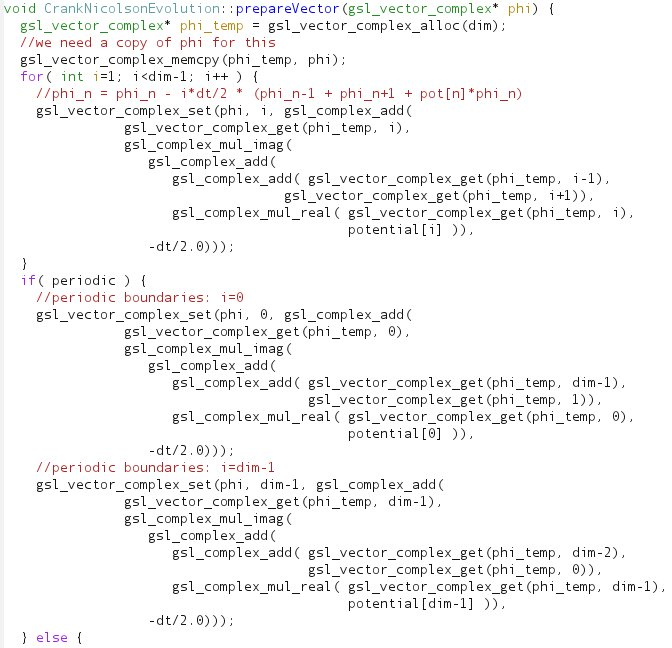
\includegraphics[draft=false,width=0.84\textwidth]{gsl_mess.jpg}
}

\frame{
  \frametitle{Portability of your algorithm}

  How to run your algorithm?
    \begin{itemize}
      \item Single machine, single CPU
      \item Single machine, multiple CPU's (OpenMP, threads, ...)
      \item Multiple machines (MPI)
      \item GPU (Cuda, Thrust, OpenCL)
    \end{itemize}

  \pause

  \vspace{2ex}

  Which data types are used by your algorithm?
   \begin{itemize}
    \item Build-in data types -- \texttt{double}, \texttt{complex<double>}
    \item Arbitrary precision types -- GMP, MPFR
    \item Vectorial data types \texttt{float2d}, \texttt{float3d}
   \end{itemize}

  \pause

  \vspace{2ex}

  \begin{block}{Theoretical solution}
    GoF Design Pattern: Strategy, also known as Policy
    
    {\tiny Gamma, Holm, Johnson, Vlissides: {\it Design Patterns, Elements of Reuseable Object-Oriented Software},  1998.}
  \end{block}
}

\frame{
  \frametitle{Numerical integration of ODEs}
  
    Find a numerical solution of an ODE an its initial value problem 
    \[ \dot{x} = f(x,t) \,\,\textrm{,} \quad \quad x(t=0) = x_0\]

   \vspace{2ex}

   Example: Explicit Euler
   \[ x(t + \Delta t ) = x(t) + \Delta t \,\, f(x(t),t) + \mathcal{O}(\Delta t^2)\]

   \vspace{2ex}

   General scheme of order $s$
    \[ x(t) \,\, \mapsto \,\, x(t+\Delta t) \quad \quad \text{, or}\]
    \[x(t + \Delta t) = \mathcal{F}_t x(t) + \mathcal{O}(\Delta t^{s+1})\]

}




\frame{
%  \frametitle{odeint - Solving ODEs in C++}

\centerline{\Large \bf \color{red}odeint}

\vspace{2ex}

\centerline{Solving ordinary differential equations in C++}

\vspace{2ex}

Open source
\begin{itemize}
\item Boost license -- do whatever you want do to with it 
\end{itemize}

\pause

\vspace{2ex}

Download
\begin{itemize}
\item \texttt{\textbf{www.odeint.com}}
% \item \texttt{https://github.com/headmyshoulder/odeint-v2}
\end{itemize}

\pause

\vspace{2ex}

Modern C++
\begin{itemize}
 \item Generic programming, functional programming 
 \item Heavy use of the C++ template system
 \item Fast, easy-to-use and extendable.
 \item Container independent
 \item Portable
\end{itemize}

}


